\chapter*{Introduction}
\label{Introduction}
\addcontentsline{toc}{chapter}{Introduction}

In the field of control systems, the inverted pendulum stands as a classic and challenging problem, serving as a benchmark for testing the capabilities of control algorithms \cite{HAMZA2019347}. This project delves into the domain of inverted pendulum dynamics, focusing on the design, simulation, and implementation of control algorithms to stabilize and control the system dynamics.

The inverted pendulum, with its inherent instability, demands precise control strategies to maintain equilibrium. Our objective is to investigate and implement four known plus one new control methodologies that not only stabilize the pendulum in its upright position but also exhibit robust performance in the face of disturbances and uncertainties.

The report encompasses the theoretical foundations of control systems for inverted pendulum. Subsequently, it delves into the specific challenges posed by inverted pendulum dynamics and the various control strategies that have been proposed in the literature such as Jezierski, Mozaryn and Suski \cite{LQRvsMPC}, book "The Inverted Pendulum in Control Theory and Robotics" \cite{bookInverted} or the book "Advanced Control of Wheeled Inverted Pendulum Systems" \cite{controlInverted}.

\begin{figure}[!tbh]
	\hfill
	\subfigure[Rotational inverted pendulum from the company quanser \cite{Quanser_2023}.]{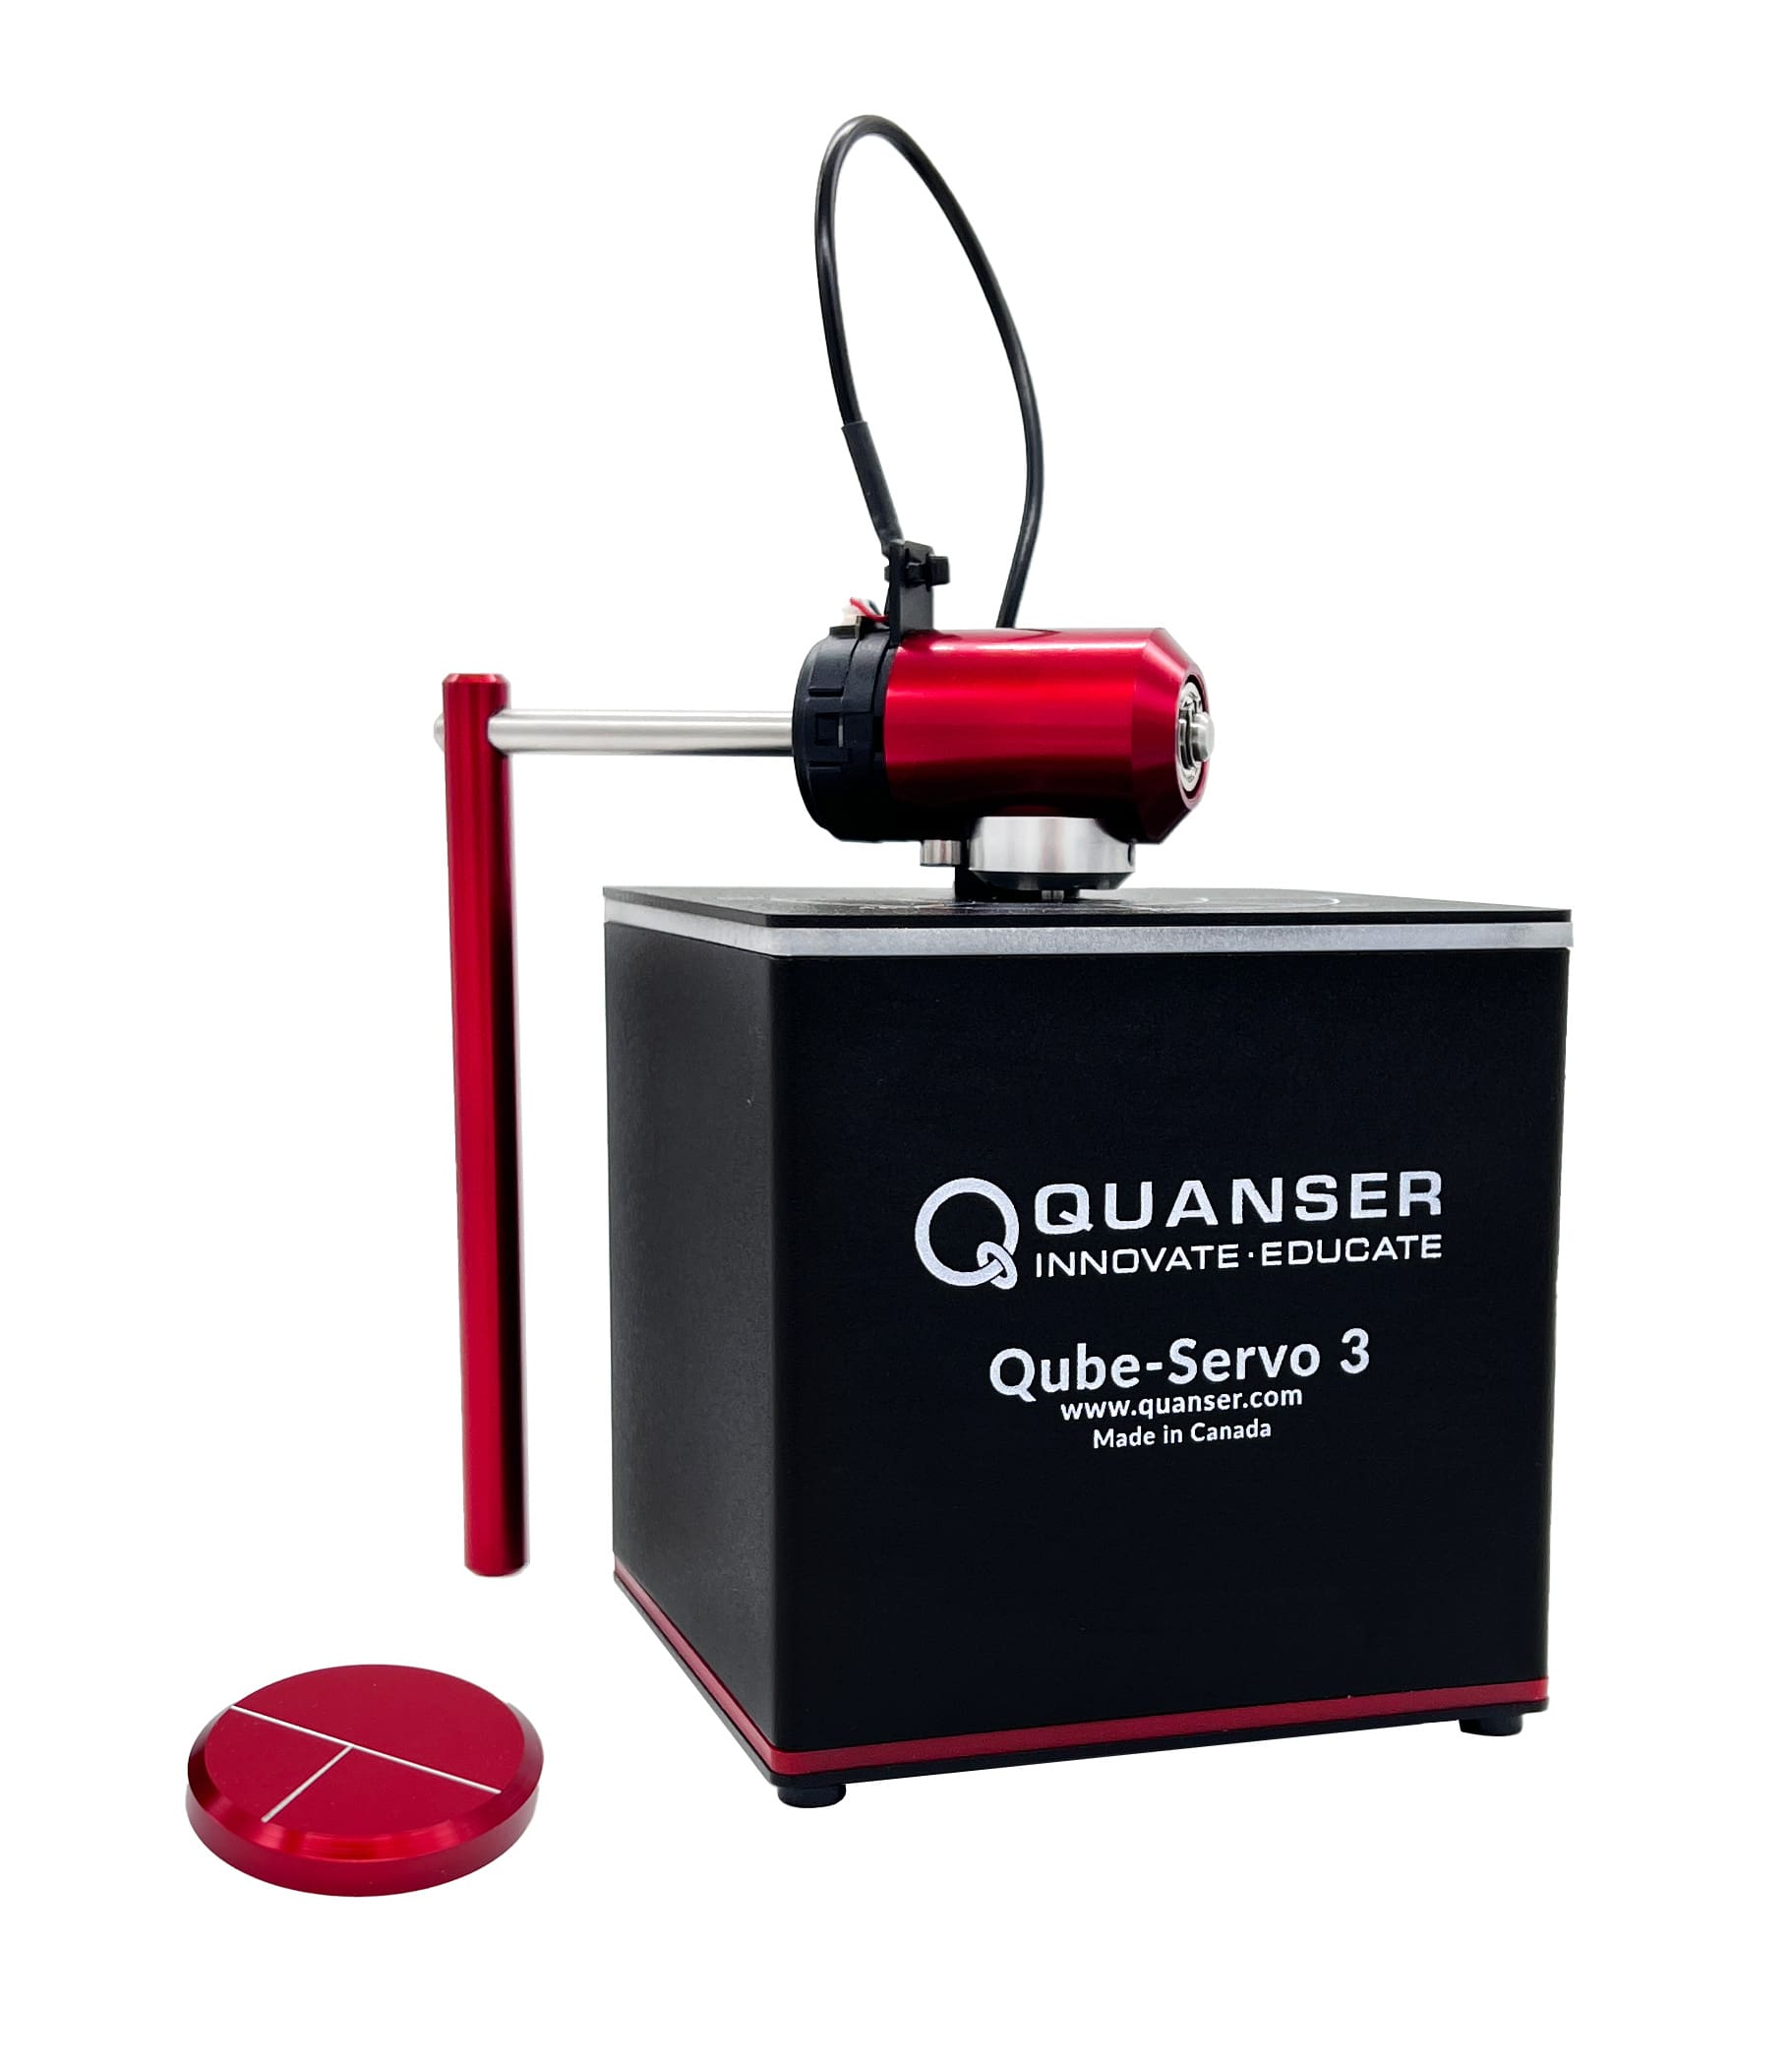
\includegraphics[width=6cm]{obr/rotationalPendulum.jpg}}
	\hfill
	\subfigure[Linear inverted pendulum from the company quanser \cite{Quanser_2023a}.]{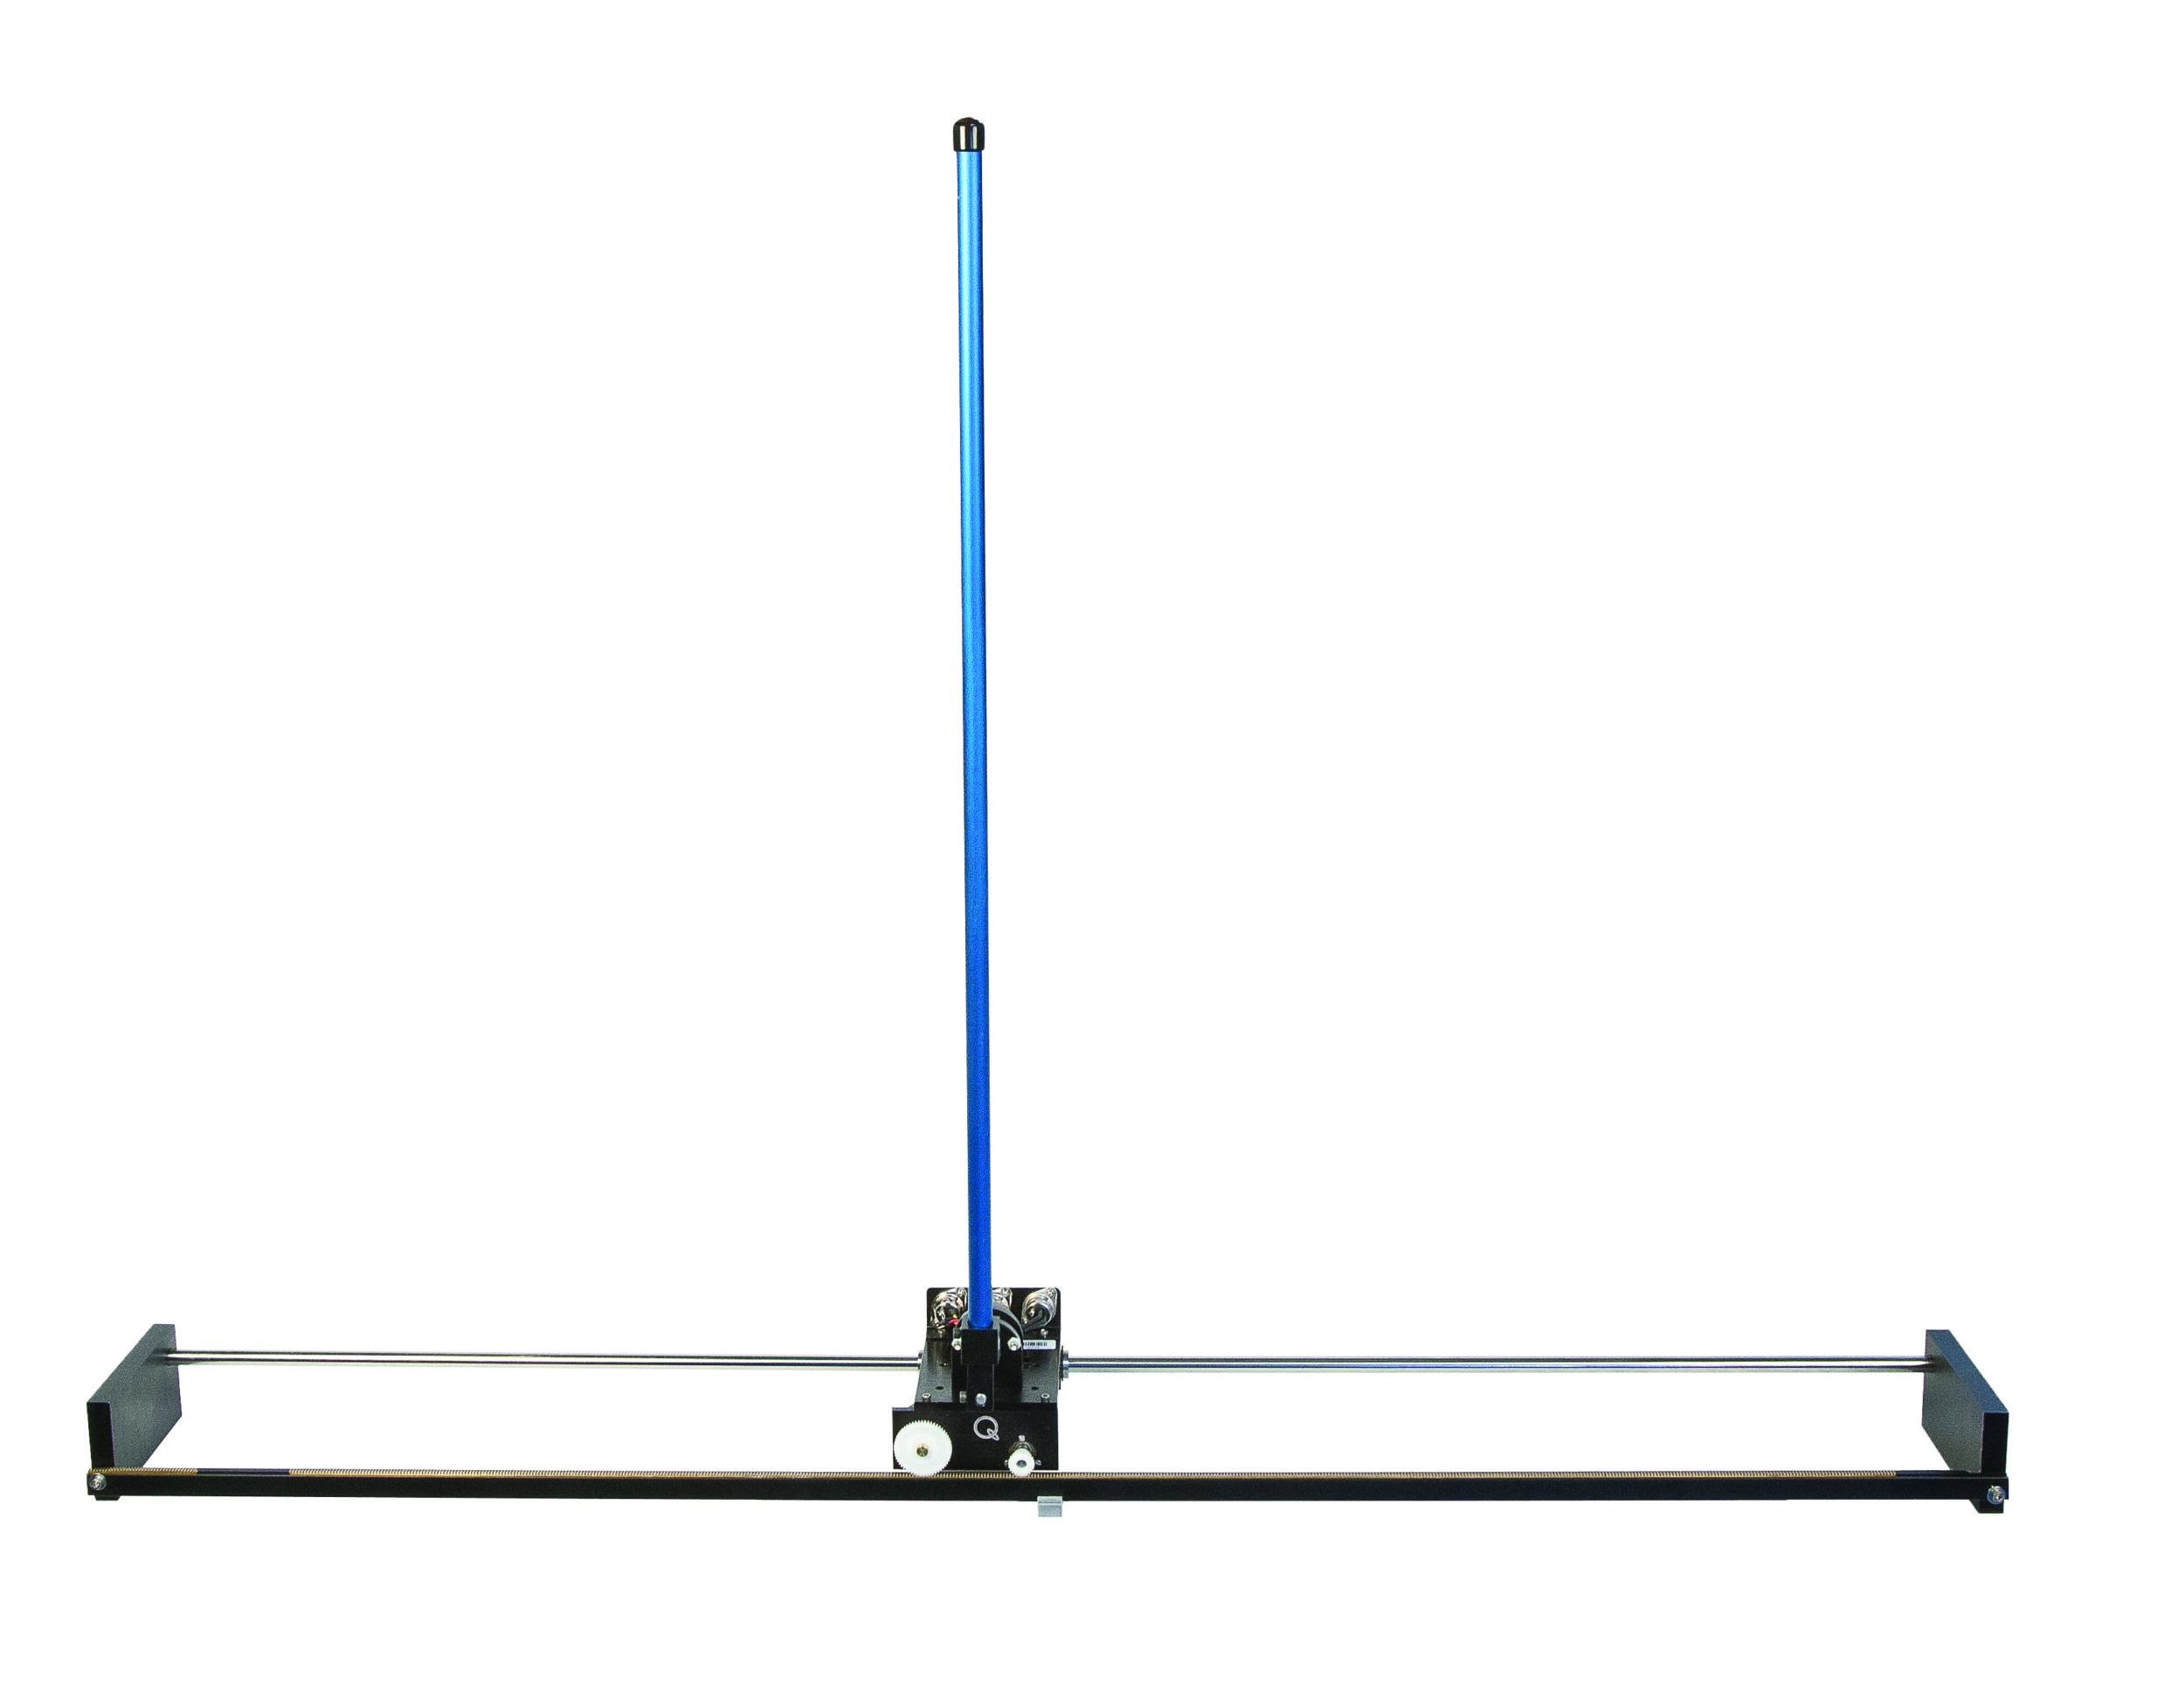
\includegraphics[width=8cm]{obr/linearPendulum.jpg}}
	\hfill
	\caption{Configurations of inverted pendulum.}\label{RotAndLin}
\end{figure}

Within the domain of inverted pendulum systems, there are two main types of configurations. It is rotational Fig. \ref{RotAndLin}.a and linear configuration Fig. \ref{RotAndLin}.b. In the case of a rotational inverted pendulum, the focus lies on managing the rotational motion of an object around a fixed pivot point. A classic example is a rigid rod attached to a pivot, and other fixed rod attached to the end of it, where the objective is to stabilize the system in an inverted position despite its inherent instability.

On the other hand, a linear inverted pendulum involves translational or linear motion along a vertical axis. This configuration is often represented by a cart on a track, with a pendulum attached to the cart. The task is to control the linear motion of the cart to maintain equilibrium with the pendulum inverted. The setup we are using for simulation and real world implementation is the linear model of inverted pendulum. 

Our focus extends beyond theoretical considerations, as the project involves practical implementation on a physical inverted pendulum setup which is located at the chair of Automation and Control of RPTU. This particular setup can be seen on the picture \ref{PICTURE_PENDULUM}. The hardware experimentation provides valuable insights into the real-world applicability of the developed algorithms, offering a bridge between theory and application.

\begin{figure}[!tbh]
	\centering
	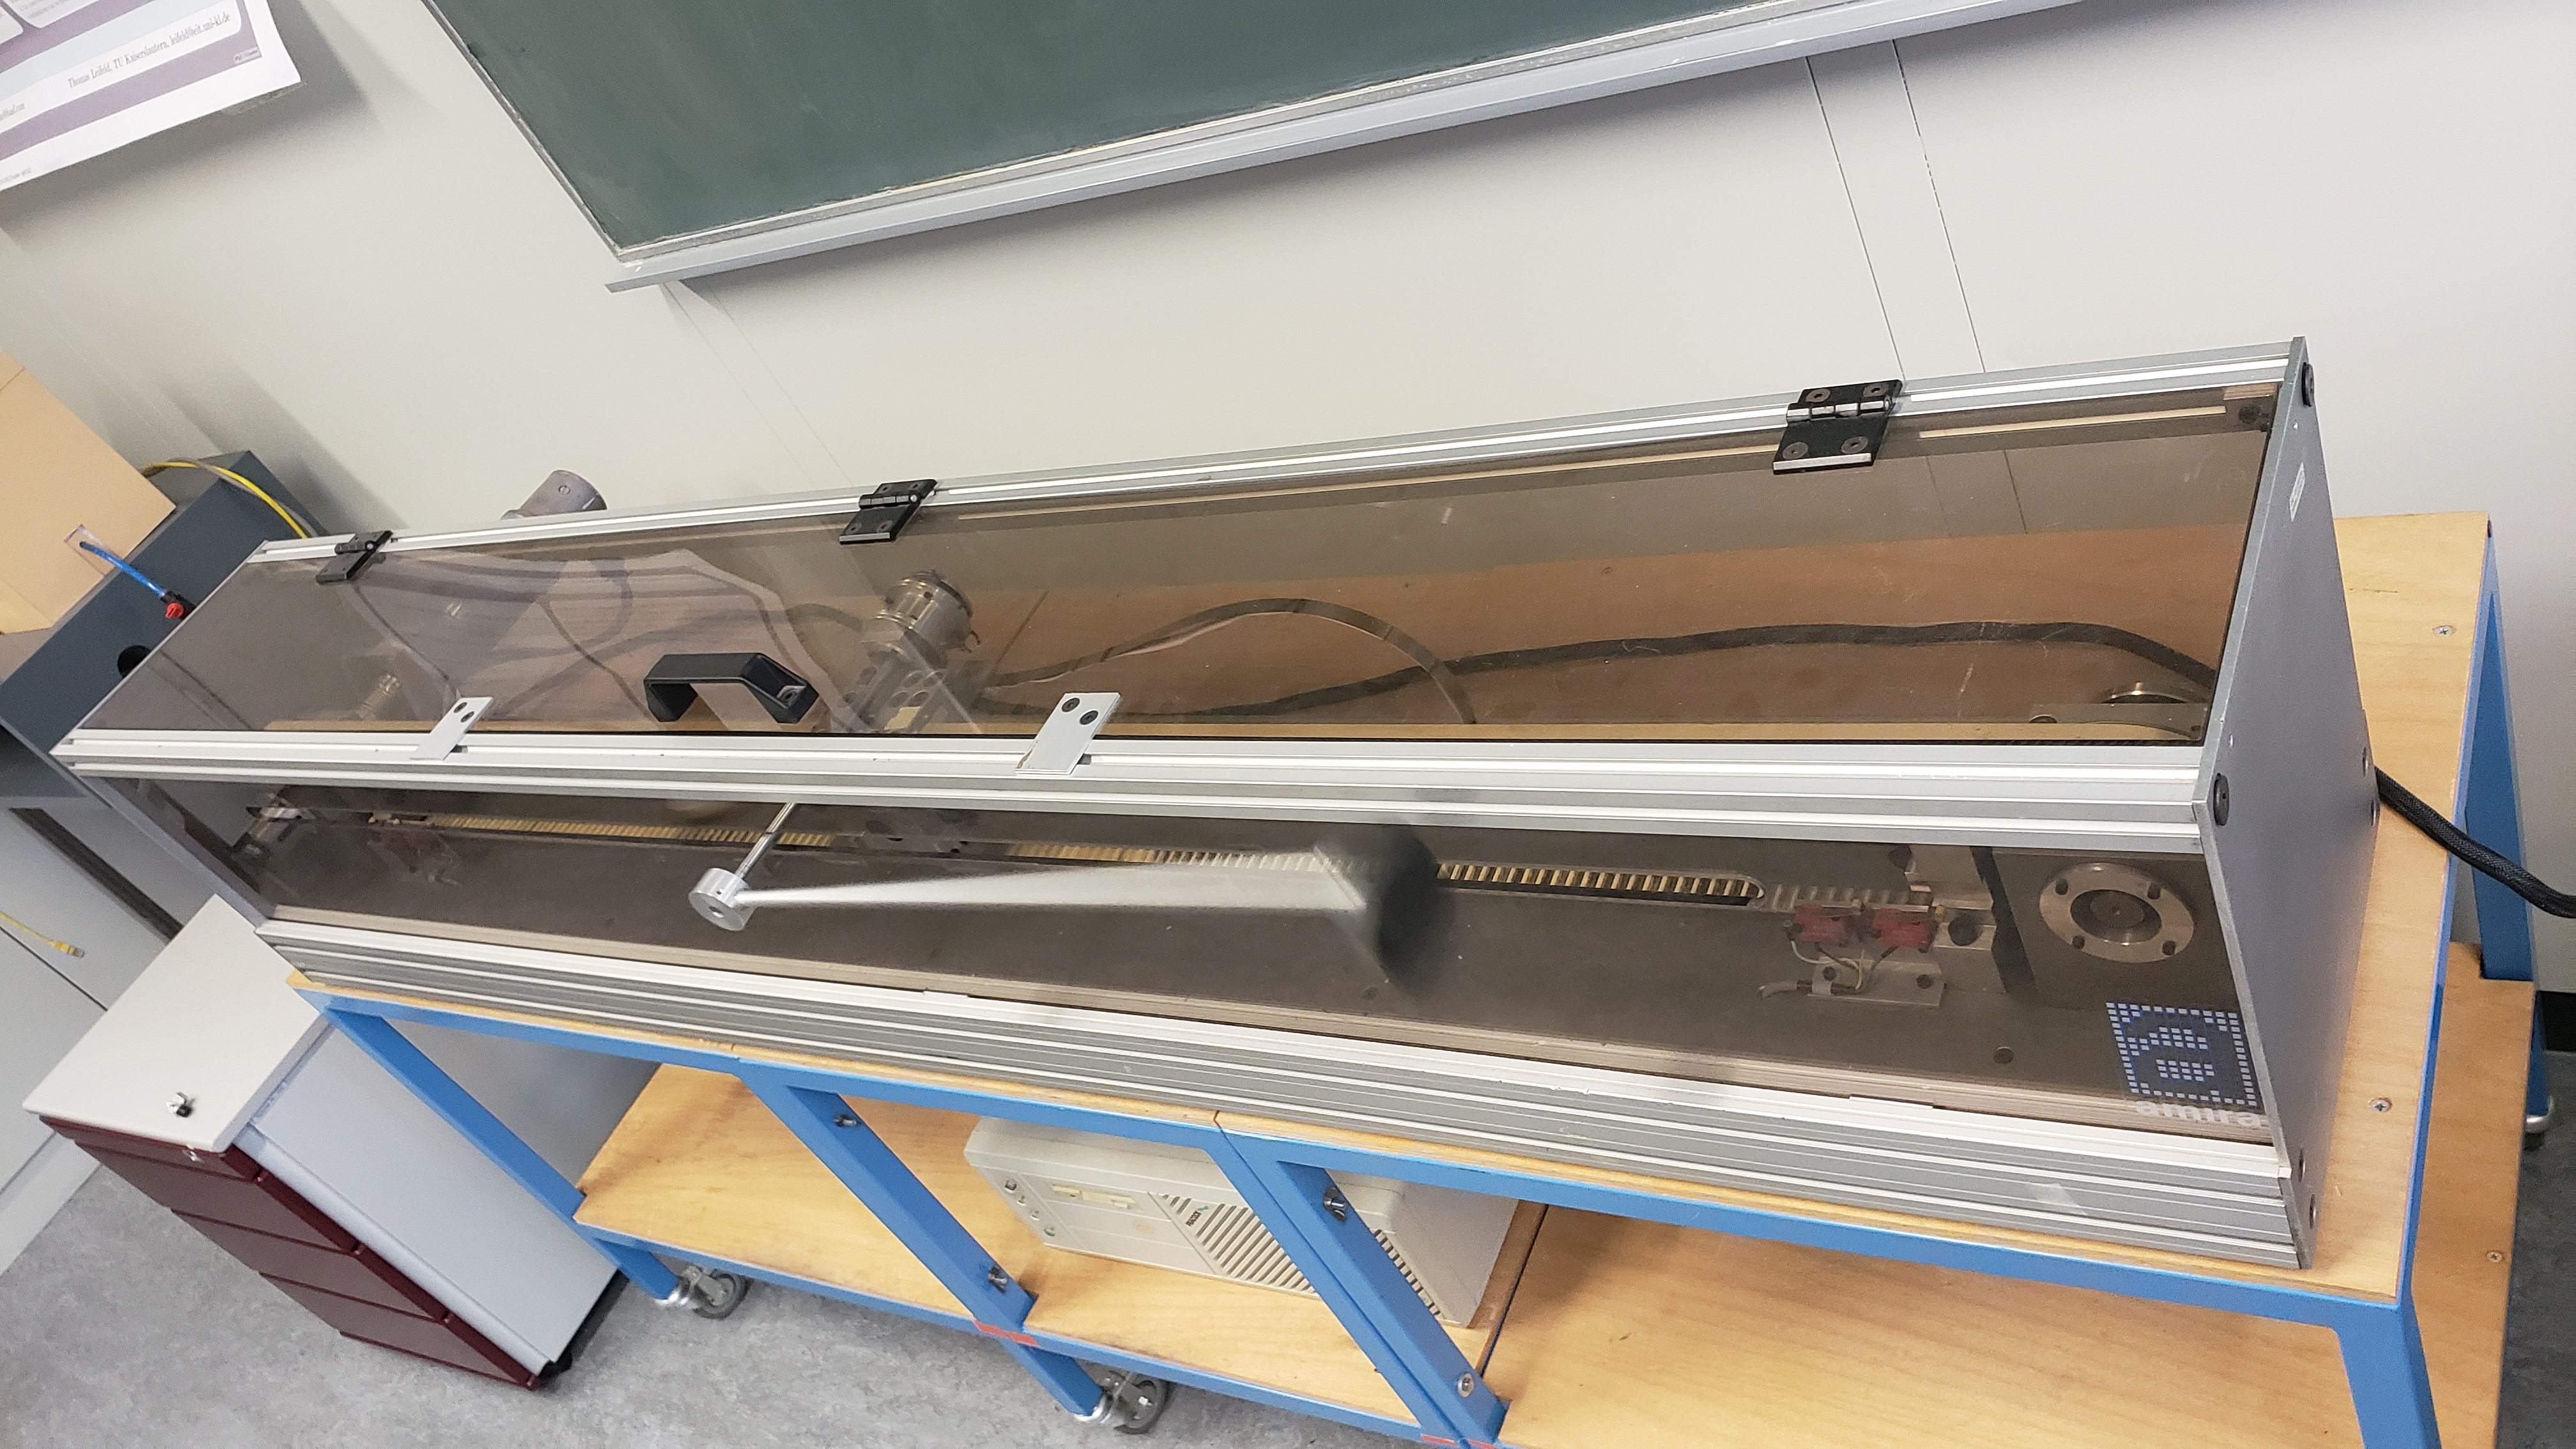
\includegraphics[width=140mm]{obr/pendulumInverted.jpg}
	\caption{Inverted pendulum setup on which implementation of designed controllers was done.}\label{PICTURE_PENDULUM}
\end{figure}

This project aims to contribute to the field of control systems by presenting a comprehensive exploration of control algorithms for inverted pendulum systems. Through rigorous analysis and experimentation, this report endeavors to showcase the effectiveness and adaptability of the implemented control algorithms, opening avenues for further advancements in the control of dynamic systems.
